\chapter{Dynamic Queries}
% structure of this chapter:
% main = dynamic queries
% Explain:
% - what I mean by that
% - basic requirements = viewer
% - beauty = can be extendend, 
%   more filetypes, not only geometry
% - 3 possible implementations, 
%   computation always in different place
% - making use of EXISTING DATA,
%   can be extended to new dedicated ontologies
This chapter introduces the concept of dynamic querying. In this thesis, it refers to the automatic generation of queries responsible for obtaining the data needed to visualize building elements from a \ac{bim} model within an \ac{rdf} graph. The examples are presented as static SPARQL queries, since the automation itself depends on the implementation or framework used. A link to the appendix is provided, where the implementation within the prototype of this thesis is explained.

The structure is as follows: first, the requirements for the viewer are researched, as its functioning will dictate the output of the queries. Second, the capabilities of the viewer are explored in relation to the visualization of semantic data, thus emphasizing the added value of working with Linked Data. Third, three types of dynamic queries for culling are presented, each with its own advantages and disadvantages.

% - importance of viewer
% - refer to state of the art existing viewers
\section{Requirements}
% - different file formats, different sources.
% - reusing first diagram
% - why XEOKIT sdk (practical)
A viewer designed to visualize data stored in an \ac{rdf} graph is required to understand the data stored within it. Therefore, the requirements for the viewer align with those of its source, the \ac{rdf} graph. Section \ref{sec:fog}, which discusses the use of both the \ac{fog} and \ac{omg} ontologies, offers an overview of the available options in terms of file format and file source. The \ac{fog} ontology supports the description of a wide range of geometry formats, as illustrated in Table \ref{tab:geometryFormats}. In conjunction with the \ac{omg} ontology, which allows for the description of the file source using the datatype of the literal, it can be concluded that the viewer should be able to handle a broad spectrum of file formats, preferably described in the \ac{fog} ontology, and accept both remote files and literal values.

\begin{table}[H]
    \centering
    \begin{tabular}{llll}
        \toprule
        COLLADA & Compressed LAS  & Compressed Nexus      & DWG      \\
        E57     & GeoJSON         & Well Known Text SFA   & GML      \\
        IFC     & IGES            & LAS Point Cloud       & Nexus    \\
        OBJ     & PCD Point Cloud & Uncompressed LAS      & Revit    \\
        Rhino   & Shapefile       & Simple Feature Access & SketchUp \\
        SPFF    & STEP SPFF       & Uncompressed Nexus    & SVG      \\
        PLY     & STL             & Well Known Binary SFA & X3D      \\
        glTF    &                 &                       &          \\ \bottomrule
    \end{tabular}
    \caption[\acs{fog} ontology geometry formats]{List of geometry formats that can be assigned with the \acs{fog} ontology.\footnotemark}
    \label{tab:geometryFormats}
\end{table}
\footnotetext{\cite{fog}}

\section{Beyond geometry}
% - possibilities of viewer extends classical approach
This section highlights the adavantages a viewer based on Linked Data has over a viewer based on traditional file-based systems, by extenting the thought of a 3D viewer to its ability to visualise non geometric data from its source. \ac{ldbim} links geometrical entities to their corresponding semantic data, which can be visualised in the viewer. This allows for the visualisation of data that is not directly related to the geometry of the building elements, such as the physical properties of a wall or the cost of a door. The possibilities are endless, as long as the data is available in the \ac{rdf} graph. The following sections will discuss different possible implementations.


\subsection{\acs{bcf} integration} \label{sec:bcf}
% - BCF viewpoints in xeokit
% - what is bcf...
As a first possible implementation of non-geometric data, this section examines the \ac{bcf} buildingSMART standard. \ac{bcf} is an open file format that enables the creation and communication of issues about \ac{bim} models \footcite{bcf}. Both it and its translation in the Semantic Web as \ac{bcfowl} \parencite{bcfOWL} link a screenshot, a camera angle, and a list of concerned entities to form a specific issue \footcite{bcfCollab}.

This type of semantic offers two types of implementations. The first is the positioning of a screenshot, together with its camera position and orientation, within the 3D scene. This allows for the visualization of issues, which can be linked to the screenshot, in the viewer, offering communication integration. The second implementation involves the metadata surrounding issues that can be used as visual properties to feed specific queries. This type of implementation is discussed in the next section, \nameref{sec:visualSemantic}.

\subsection{Visualising semantic} \label{sec:visualSemantic}
% - element associated data
% - physical: thermal, acoustic, ...
% - non-physical: cost, time, pothologies, ...
% - all  with temporal dimension / history
When examining semantics such as physical properties of entities, free from geometric and spatial data (see \nameref{sec:bcf}), a visual interpretation superimposed on the viewer offers powerful rendering possibilities. By coloring elements based on their properties, both physical and non-physical, the viewer can be used to detect anomalies or insights in the model, in a feature-rich output medium.

Physical properties such as thermal, acoustic, structural, and others, or non-physical properties like cost, time, and pathologies, can all be described and linked in the \ac{rdf} graph. The expressive capabilities of \ac{sparql} enable complex and fine-grained queries, offering application-specific query creation about these properties. By selecting a specific subset or combining them, a user or developer can transform the viewer into a powerful tool.

As such, the viewer is expected to comply with a multitude of requirements, which are not all covered in this thesis. Chapter \nameref{ch:modularApproach} thus proposes a modular approach, allowing for a step-by-step implementation of the viewer, starting with the most basic requirements, which are adopted in Chapter \nameref{ch:prototype}, while leaving room for future extensions.

\section{In situ WKT location}
% - limited to 2D
% - viewer: knows location, AR: knnows 
% - on building site location system 
%   / BIM model translated into WKT literals in model
% - use of WKT and GeoSPARQL
% - to which extends needs every element a location
% - which queries are possible
The first type of dynamic query identifies the room in which the observer/camera is located using the \ac{wkt} serialization of \mintinline{sparql}|bot:Space| entities. It proposes to base its culling algorithm on super-elements such as rooms, thus grouping the scene into a limited number of elements within meaningful boundaries. As entities are primarily viewed within their allocated rooms, this approach takes advantage of the spatial organization of buildings using the \ac{bot} ontology. Moreover, not all building elements have a meaningful \ac{wkt} serialization (e.g., a door), which makes the use of super-elements necessary.

This approach is limited to 2D, as the widely adopted GeoSPARQL functions used to achieve this are constrained to 2D. Nonetheless, the approach can be extended to 3D if the GeoSPARQL functions are extended to 3D in the future or the needed introduction of a 3D \ac{sparql} is adopted.

Listing \ref{lst:GeoSPARQLauto} proposes a static query in which firstly a location is assigned to the variable \mintinline{sparql}|?location| to create an easily reusable query. This location is the \ac{wkt} serialization of a point, of which the coordinates can be updated at each move of the camera in the viewer. It therefore represents the location of the observer both on site, in situ for augmented reality usecases, as in the 3D scene. 

The query then combines two sets of so called entities, represented in the graph as \mintinline{sparql}|bot:Element| or \mintinline{sparql}|bot:Space|, both are linked in the graph to their corresponding \ac{wkt} and geometric serialization using an \ac{omg} level 1 pattern. This pattern level links the literal directly to the entity, without the need of an intermediate node, but without the possibility to assign multiple serialisations of the same type. The geometry literal is assigned using the \ac{fog} ontology, while the \ac{wkt} literal is assigned using the GeoSPARQL ontology. As this last serialization requires a \ac{wkt} format, a literal assigned with \mintinline{sparql}|geo:asWKT| is required, and queried for in the query. 

The separation in two sets lets both query for entities that have a \ac{wkt} serialization but are not located in a \mintinline{sparql}|bot:Space| and entities that are located in a \mintinline{sparql}|bot:Space| that have a \ac{wkt} serialization but themselves do not have a \ac{wkt} serialization. The latter variant uses the \mintinline{sparql}|bot:containsElement| property to select entities within a room.

After filtering out spaces, of which the geometry is not  needed by the viewer, it filters objects geometry based on a list of implemented / accepted formats by the receiving viewer. 


\begin{figure}[H]
    \begin{adjustwidth}{-0.8cm}{-0.8cm}
        \centering
        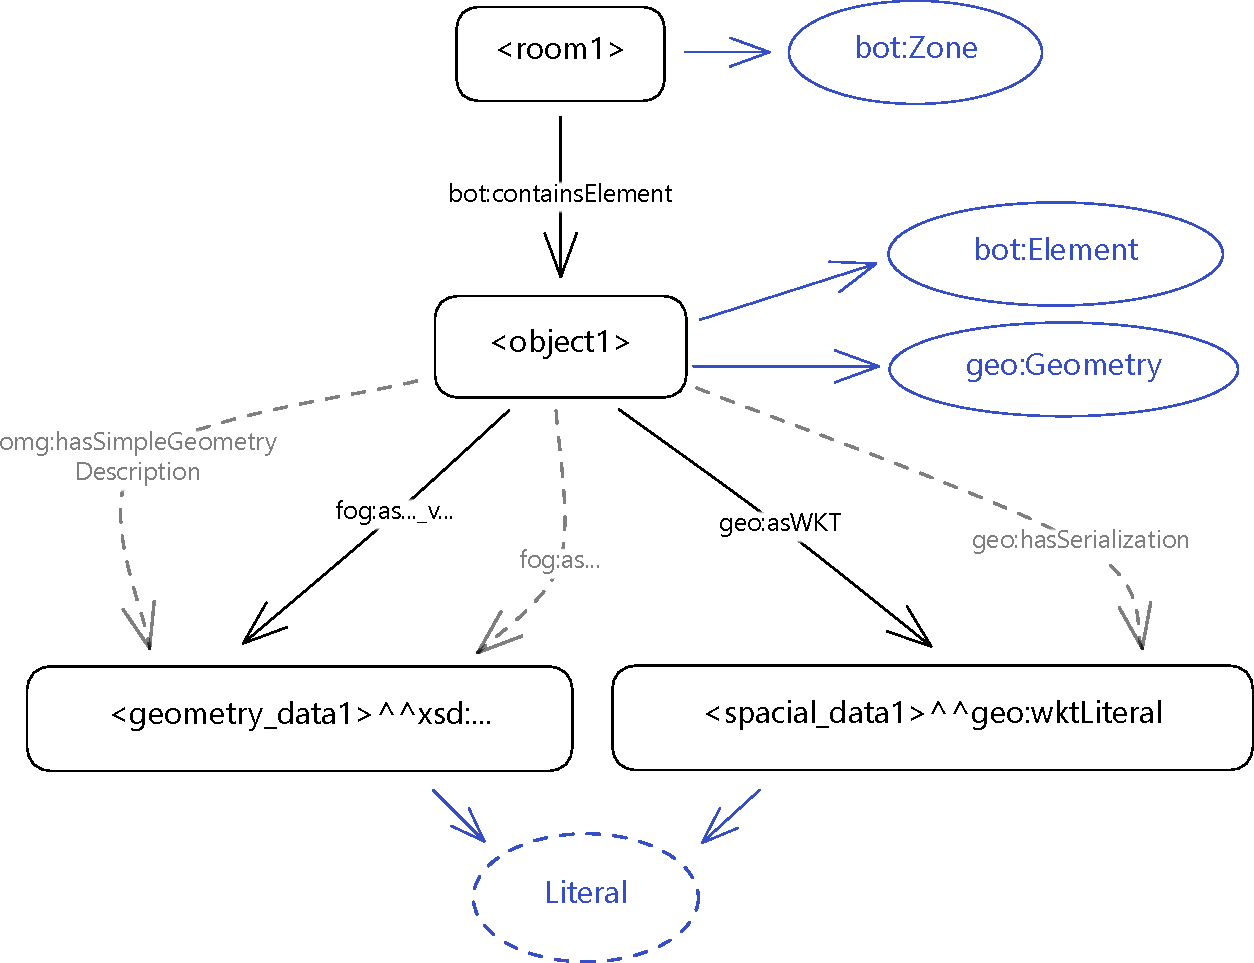
\includegraphics[width=0.8\textwidth]{figures/pdf/omg1.pdf}
        \caption{omg1}
        \label{fig:omg1}
    \end{adjustwidth}
\end{figure}


% query by distance, instance instead adjacent

\begin{listing}[H]
    \inputminted{sparql}{dynamicQueries/inSitu/query.rq}
    \vspace{-0.7cm}
    \caption{Dynamic culling query using GeoSPARQL}
    \label{lst:GeoSPARQLauto}
\end{listing}


\section{In viewer "bot:Space" identification}
% - 1 database + 1 3D enabled instance (viewer) 
%   => viewer can raytrace identify wright space (little computation)
% - 2 layered viewer visible elements / invisible spaces
% - sequence diagram
%   - manual first step + adjacent spaces
%   - all spaces
%   - combination of spaces
% - sample queries

\begin{listing}[H]
    \inputminted{sparql}{dynamicQueries/inViewer/query.rq}
    \vspace{-0.7cm}
    \caption{Querying in viewer "bot:Space" identification}
    \label{lst:BOTauto}
\end{listing}


\section{In query OBJ geometry filtering}
% - no geometric but string analysis in query
% - AABBox filtering of for example obj rooms
% - all negative points

\begin{listing}[H]
    \inputminted{sparql}{dynamicQueries/inQuery/query.rq}
    \vspace{-0.7cm}
    \caption{Querying in query OBJ geometry filtering}
    \label{lst:OBJauto}
\end{listing}

\begin{listing}[H]
    \inputminted{js}{dynamicQueries/inQuery/function.js}
    \vspace{-0.7cm}
    \caption{Querying in situ WKT location}
    \label{lst:OBJautoFunction}
\end{listing}

